%%%%%%%%%%%%%%%%%%%%%%%%%%%%%%%%%%%%%%%%%
% Beamer Presentation
% LaTeX Template
% Version 1.0 (10/11/12)
%
% This template has been downloaded from:
% http://www.LaTeXTemplates.com
%
% License:
% CC BY-NC-SA 3.0 (http://creativecommons.org/licenses/by-nc-sa/3.0/)
%
%%%%%%%%%%%%%%%%%%%%%%%%%%%%%%%%%%%%%%%%%

%----------------------------------------------------------------------------------------
%	PACKAGES AND THEMES
%----------------------------------------------------------------------------------------

\documentclass{beamer}

\mode<presentation> {

% The Beamer class comes with a number of default slide themes
% which change the colors and layouts of slides. Below this is a list
% of all the themes, uncomment each in turn to see what they look like.

%\usetheme{default}
%\usetheme{AnnArbor}
%\usetheme{Antibes}
%\usetheme{Bergen}
%\usetheme{Berkeley}
%\usetheme{Berlin}
%\usetheme{Boadilla}
%\usetheme{CambridgeUS}
%\usetheme{Copenhagen}
%\usetheme{Darmstadt}
%\usetheme{Dresden}
%\usetheme{Frankfurt}
%\usetheme{Goettingen}
%\usetheme{Hannover}
%\usetheme{Ilmenau}
%\usetheme{JuanLesPins}
%\usetheme{Luebeck}
\usetheme{Madrid}
%\usetheme{Malmoe}
%\usetheme{Marburg}
%\usetheme{Montpellier}
%\usetheme{PaloAlto}
%\usetheme{Pittsburgh}
%\usetheme{Rochester}
%\usetheme{Singapore}
%\usetheme{Szeged}
%\usetheme{Warsaw}

% As well as themes, the Beamer class has a number of color themes
% for any slide theme. Uncomment each of these in turn to see how it
% changes the colors of your current slide theme.

%\usecolortheme{albatross}
%\usecolortheme{beaver}
%\usecolortheme{beetle}
%\usecolortheme{crane}
%\usecolortheme{dolphin}
%\usecolortheme{dove}
%\usecolortheme{fly}
%\usecolortheme{lily}
%\usecolortheme{orchid}
%\usecolortheme{rose}
%\usecolortheme{seagull}
%\usecolortheme{seahorse}
%\usecolortheme{whale}
%\usecolortheme{wolverine}

%\setbeamertemplate{footline} % To remove the footer line in all slides uncomment this line
%\setbeamertemplate{footline}[page number] % To replace the footer line in all slides with a simple slide count uncomment this line

%\setbeamertemplate{navigation symbols}{} % To remove the navigation symbols from the bottom of all slides uncomment this line
}

\usepackage{graphicx} % Allows including images
\usepackage{booktabs} % Allows the use of \toprule, \midrule and \bottomrule in tables

\usepackage{tikz}
\usepackage{pgfplots}
%----------------------------------------------------------------------------------------
%	TITLE PAGE
%----------------------------------------------------------------------------------------

\title[]{} % The short title appears at the bottom of every slide, the full title is only on the title page

\author{D.D., A.R.} % Your name
\institute[] % Your institution as it will appear on the bottom of every slide, may be shorthand to save space
{ \\ % Your institution for the title page
\medskip
\textit{} % Your email address
}
\date{\today} % Date, can be changed to a custom date

\begin{document}

%\begin{frame}
%\titlepage % Print the title page as the first slide
%\end{frame}

%\begin{frame}
%\frametitle{Overview} % Table of contents slide, comment this block out to remove it
%\tableofcontents % Throughout your presentation, if you choose to use \section{} and \subsection{} commands, these will automatically be printed on this slide as an overview of your presentation
%\end{frame}

%----------------------------------------------------------------------------------------
%	PRESENTATION SLIDES
%----------------------------------------------------------------------------------------

%------------------------------------------------
\section{First Section} % Sections can be created in order to organize your presentation into discrete blocks, all sections and subsections are automatically printed in the table of contents as an overview of the talk
%------------------------------------------------

\subsection{Subsection Example} % A subsection can be created just before a set of slides with a common theme to further break down your presentation into chunks

\begin{frame}
\frametitle{Multi-level by knot insertion}

\begin{itemize}
	\item Consider the multi-level for IGA:
	\begin{itemize}
		\item Start from a base knot-vector.
		\item Super-imposition of knot-vectors obtained by knot insertion.
	\end{itemize}
	\item Knot insertion defines a space containing the space defined by the previous knot-vector.
	\begin{itemize}
		\item "Nested spaces"
	\end{itemize}
	\item Recursively: it contains the space defined by \textbf{all} previous knot vectors.
\end{itemize}
\centering
\includegraphics[scale=0.175]{operators1d/multiLevelBasis.png}
\end{frame}

\begin{frame}
	\frametitle{Multi-level by knot insertion}
	
	\begin{itemize}
	\item $ \implies $ Linear combination of basis function of one level can represent all the basis functions of all the level below it.
	\item $ N^1 = M^{12} N^2 $.
	\item $ M^{12} $ is a standard knot insertion matrix available in the literature.%
%	\item If knot vector of levels 2 is obtained by repeating all knots to get c0-continuity
%	\begin{itemize}
%		\item then $ M^{12} $  is the B\`ezier Extraction Operator
%\end{itemize}

\end{itemize}
	\includegraphics[width=0.57\textwidth]{pics/refinement.png}%
	\hspace{-1.8cm}%
	\includegraphics[width=0.57\textwidth]{pics/refinementf.png}
\end{frame}

\begin{frame}
	\frametitle{Multi-level by knot insertion}
	\begin{itemize}
		\item The $  M^{mn} $ operator can be localized to each knot-span
			\begin{itemize}
				\item "Element point of view"
			\end{itemize}
		\item $ N_e^1 = M_e^{12} N_e^2 $.
	\end{itemize}
	\centering
	\includegraphics[scale=0.23]{operators1d/multiLevelBasis.png}

\end{frame}

\begin{frame}
	\frametitle{Multi-level Operator}
		 These properties are exploited to ease the implementation of multi-level refinements
		\begin{itemize}
			\item First: define active leaf-elements on each levels
		\end{itemize}
		
		
		\includegraphics[width=\textwidth]{operators1d/multiLevelBasis.png}
		
\end{frame}


\begin{frame}
	\frametitle{Multi-level Operator}
	\begin{itemize}
		\item Second: identify active ( dashed and solid) and non-active (dotted and gray) basis functions
	\end{itemize}
	
	
	\includegraphics[width=\textwidth]{operators1d/multiLevelBasis.png}
	
\end{frame}



\begin{frame}
	\frametitle{Multi-level Operator}
	\begin{itemize}
		\item For each (leaf-)element, compute the linear operator that relates the non-zero functions on the element (active and non-active) to the non-zero active functions of \textbf{all} previous levels
	\end{itemize}
	\centering
	\includegraphics[scale=0.22]{operators1d/multiLevelBasis.png}
	
\end{frame}

%\begin{frame}
%	\frametitle{Multi-level Operator}
%		E.g., for the 4th element from left\\
%		%\item $ N_e^{\textit{all}} = M_e \tilde {N}_e^3 $.
%		$ \underset{\scriptscriptstyle \textcolor{gray}{5x1}}{N_e^{\textit{all}}} =  \begin{bmatrix}
%		\vspace{0.15cm}
%		\underset{\scriptscriptstyle \textcolor{gray}{3x1}}{\textcolor{blue}{N^1_e}}  \\
%		\vspace{0.15cm}
%		\underset{\scriptscriptstyle \textcolor{gray}{1x1}}{\textcolor{green}{N^2_e}}  \\
%		\underset{\scriptscriptstyle \textcolor{gray}{1x1}}{\textcolor{red}{N^3_e}}  \\
%		\end{bmatrix} = \begin{bmatrix}
%		\vspace{0.15cm}
%		\underset{\scriptscriptstyle \textcolor{gray}{3x4}}{M^{13}_e}  \underset{\scriptscriptstyle \textcolor{gray}{4x1}}{\textcolor{red}{\tilde N^3_e}} \\
%		\vspace{0.15cm}
%		\underset{\scriptscriptstyle \textcolor{gray}{1x4}}{M^{12}_e} \underset{\scriptscriptstyle \textcolor{gray}{4x1}}{\textcolor{red}{\tilde N^3_e}} \\
%		\underset{\scriptscriptstyle \textcolor{gray}{1x4}}{I^{3}_{active}} \underset{\scriptscriptstyle \textcolor{gray}{4x1}}{\textcolor{red}{\tilde N^3_e}}   \\
%		\end{bmatrix}= \begin{bmatrix}
%		\vspace{0.15cm}
%		\underset{\scriptscriptstyle \textcolor{gray}{3x4}}{M^{13}_e}   \\
%		\vspace{0.15cm}
%		\underset{\scriptscriptstyle \textcolor{gray}{1x4}}{M^{12}_e}  \\
%		\underset{\scriptscriptstyle \textcolor{gray}{1x4}}{I^{3}_{active}}   \\
%		\end{bmatrix} \underset{\scriptscriptstyle \textcolor{gray}{4x1}}{\textcolor{red}{\tilde N^3_e}} = 
%		\underset{\scriptscriptstyle \textcolor{gray}{5x4}}{M_e} \underset{\scriptscriptstyle \textcolor{gray}{4x1}}{\textcolor{red}{\tilde N^3_e}} $	
%	Where \begin{itemize}
%		\item  $ \textcolor{red}{N^3_e} $: \emph{active} functions (solid and dashed) on element 
%		\item  $ \textcolor{red}{\tilde N^3_e} $: \emph{active and non-active} functions (solid, dashed, dotted) on elem.
%		\item $ I^{3}_{active} $: selects the active basis functions $ \textcolor{red}{N^3_e}= I^{3}_{active}\textcolor{red}{\tilde N^3_e} $
%	\end{itemize}
%	\includegraphics[width=\textwidth]{operators1d/multiLevelBasis.png}
%	
%\end{frame}
%
%\begin{frame}
%	\frametitle{Multi-level Operator}
%	%\item $ N_e^{\textit{all}} = M_e \tilde {N}_e^3 $.
%	$ \underset{\scriptscriptstyle \textcolor{gray}{5x1}}{N_e^{\textit{all}}} =  \begin{bmatrix}
%	\vspace{0.15cm}
%	\underset{\scriptscriptstyle \textcolor{gray}{3x1}}{\textcolor{blue}{N^1_e}}  \\
%	\vspace{0.15cm}
%	\underset{\scriptscriptstyle \textcolor{gray}{1x1}}{\textcolor{green}{N^2_e}}  \\
%	\underset{\scriptscriptstyle \textcolor{gray}{1x1}}{\textcolor{red}{N^3_e}}  \\
%	\end{bmatrix} = \begin{bmatrix}
%	\vspace{0.15cm}
%	\underset{\scriptscriptstyle \textcolor{gray}{3x4}}{M^{13}_e}  \underset{\scriptscriptstyle \textcolor{gray}{4x1}}{\textcolor{red}{\tilde N^3_e}} \\
%	\vspace{0.15cm}
%	\underset{\scriptscriptstyle \textcolor{gray}{1x4}}{M^{12}_e} \underset{\scriptscriptstyle \textcolor{gray}{4x1}}{\textcolor{red}{\tilde N^3_e}} \\
%	\underset{\scriptscriptstyle \textcolor{gray}{1x4}}{I^{3}_{active}} \underset{\scriptscriptstyle \textcolor{gray}{4x1}}{\textcolor{red}{\tilde N^3_e}}   \\
%	\end{bmatrix}= \begin{bmatrix}
%	\vspace{0.15cm}
%	\underset{\scriptscriptstyle \textcolor{gray}{3x4}}{M^{13}_e}   \\
%	\vspace{0.15cm}
%	\underset{\scriptscriptstyle \textcolor{gray}{1x4}}{M^{12}_e}  \\
%	\underset{\scriptscriptstyle \textcolor{gray}{1x4}}{I^{3}_{active}}   \\
%	\end{bmatrix} \underset{\scriptscriptstyle \textcolor{gray}{4x1}}{\textcolor{red}{\tilde N^3_e}} = 
%	\underset{\scriptscriptstyle \textcolor{gray}{5x4}}{M_e} \underset{\scriptscriptstyle \textcolor{gray}{4x1}}{\textcolor{red}{\tilde N^3_e}} $	
%	Where \begin{itemize}
%		\item  $ \textcolor{red}{N^3_e} $: \emph{active} functions (solid and dashed) on element 
%		\item  $ \textcolor{red}{\tilde N^3_e} $: \emph{active and non-active} functions (solid, dashed, dotted) on elem.
%		\item $ I^{3}_{active} $: selects the active basis functions $ \textcolor{red}{N^3_e}= I^{3}_{active}\textcolor{red}{\tilde N^3_e} $
%	\end{itemize}
%	\includegraphics[width=\textwidth]{operators1d/multiLevelBasis.png}
%	
%\end{frame}

\begin{frame}
	\frametitle{Multi-level Operator}
	{\small
	E.g., for the 5th element from left\\
	$ \underset{\scriptscriptstyle \textcolor{gray}{6x1}}{N_e} =  \begin{bmatrix}
	\vspace{0.15cm}
	\underset{\scriptscriptstyle \textcolor{gray}{3x1}}{\textcolor{blue}{N^1_e}}  \\
	\vspace{0.15cm}
	\underset{\scriptscriptstyle \textcolor{gray}{1x1}}{\textcolor{green}{N^2_e}}  \\
	\underset{\scriptscriptstyle \textcolor{gray}{2x1}}{\textcolor{red}{N^3_e}}  \\
	\end{bmatrix} = \begin{bmatrix}
	\vspace{0.15cm}
	\underset{\scriptscriptstyle \textcolor{gray}{3x4}}{M^{13}_e}  \underset{\scriptscriptstyle \textcolor{gray}{4x1}}{\textcolor{red}{\tilde N^3_e}} \\
	\vspace{0.15cm}
	\underset{\scriptscriptstyle \textcolor{gray}{1x4}}{M^{12}_e} \underset{\scriptscriptstyle \textcolor{gray}{4x1}}{\textcolor{red}{\tilde N^3_e}} \\
	\underset{\scriptscriptstyle \textcolor{gray}{2x4}}{I^{3}_{active}} \underset{\scriptscriptstyle \textcolor{gray}{4x1}}{\textcolor{red}{\tilde N^3_e}}   \\
	\end{bmatrix}= \begin{bmatrix}
	\vspace{0.15cm}
	\underset{\scriptscriptstyle \textcolor{gray}{3x4}}{M^{13}_e}   \\
	\vspace{0.15cm}
	\underset{\scriptscriptstyle \textcolor{gray}{1x4}}{M^{12}_e}  \\
	\underset{\scriptscriptstyle \textcolor{gray}{2x4}}{I^{3}_{active}}\\
	\end{bmatrix} \underset{\scriptscriptstyle \textcolor{gray}{4x1}}{\textcolor{red}{\tilde N^3_e}} = 
	\underset{\scriptscriptstyle \textcolor{gray}{6x4}}{M_e} \underset{\scriptscriptstyle \textcolor{gray}{4x1}}{\textcolor{red}{\tilde N^3_e}} $	\\
\begin{itemize}
		\item  $ \textcolor{red}{N^3_e} $: \emph{active} functions (solid and dashed) on element 
		\item  $ \textcolor{red}{\tilde N^3_e} $: \emph{active and non-active} functions (solid, dashed, dotted) on element
		\item $ I^{3}_{active} $: selects the active basis functions $ \textcolor{red}{N^3_e}= I^{3}_{active}\textcolor{red}{\tilde N^3_e} $
	\end{itemize}
}
	\centering
	\begin{minipage}{0.48\textwidth}
		\centering
\includegraphics[scale=0.159]{operators1d/multiLevelBasis.png}
	\end{minipage}
	\hfill
		\begin{minipage}{0.48\textwidth}
			\centering
		\tiny	
$  M_e = \left[\begin{smallmatrix}
    \textcolor{blue}{0.0156}  &       \textcolor{blue}{0}   &      \textcolor{blue}{0}   &      \textcolor{blue}{0}\\
    \textcolor{blue}{0.4844}  &  \textcolor{blue}{0.3125}  &  \textcolor{blue}{0.1562}   & \textcolor{blue}{0.0625}\\
    \textcolor{blue}{0.4844} &   \textcolor{blue}{0.6250}   & \textcolor{blue}{0.6875}  &\textcolor{blue}{0.6250}\\
    \textcolor{green}{0.1250} &   \textcolor{green}{ 0.5000} &   \textcolor{green}{0.7500}  &   \textcolor{green}{0.5000}\\
    \textcolor{red}{0}       &  \textcolor{red}{0}   & \textcolor{red}{1}      &   \textcolor{red}{0}\\
    \textcolor{red}{0}       &  \textcolor{red}{0}   &      \textcolor{red}{0}  &  \textcolor{red}{1}\\
	\end{smallmatrix} \right]
  $
		\end{minipage}
	
	
\end{frame}



%\begin{frame}
%	\frametitle{Multi-level Operator}
%	These properties are exploited to ease the implementation of multi-level refinements
%	\begin{itemize}
%		\item First: define active leaf-elements on each levels
%		\item Second: define active and non active basis functions
%		\item For each leaf:
%		\begin{itemize}
%			\item Compute linear operator that expresses all the active shapes of all previous elements
%			\begin{itemize}
%				\item $ N_e^{\textit{all}} = M_e N_e^3 $.
%				\item See white board
%			\end{itemize}
%			\item To have full localization, combine with B\`ezier Extraction Operator $ C $
%			\begin{itemize}
%				\item $ N_e^{\textit{all}} = M_e N_e^3 = M_e C^3_e B_e $.
%				\item See examples
%			\end{itemize}
%		\end{itemize}
%	\end{itemize}
%	
%\end{frame}

\begin{frame}
	\frametitle{Multi-level B\`ezier Extraction Operator}
	\begin{itemize}
			\item To ease implementation on FEM codes, combine with B\`ezier Extraction Operator $ C $
			\begin{itemize}
				\item $ N_e^{\textit{all}} = M_e N_e^3 = M_e C^3_e B_e = K_e B_e$.
			\end{itemize}
	\end{itemize}
	
	
	\includegraphics[width=\textwidth]{operators1d/multiLevelBasis.png}
	
\end{frame}

\begin{frame}
	\frametitle{Multi-level B\`ezier Extraction Operator}
	\begin{itemize}
		\item Truncation can be included in the operator $ M_e $ by considering in each level just the linear combination of the dotted functions.
		\item I.e., the rows and columns of active functions are set to zero in each level.
	\end{itemize}
	
		\centering
		\begin{minipage}{0.78\textwidth}
			\centering
			\includegraphics[scale=0.205]{operators1d/THBS.png}
		\end{minipage}
		\begin{minipage}{0.21\textwidth}
			\tiny%
	\centering	
$ M_e= \left[\begin{smallmatrix}
\textcolor{blue}{0.0156}  &       \textcolor{blue}{0}   &      \textcolor{blue}{0}   &      \textcolor{blue}{0}\\
\textcolor{blue}{0.4844}  &  \textcolor{blue}{0.3125}  &  \textcolor{blue}{0.1562}   & \textcolor{blue}{0.0625}\\
\textcolor{blue}{0.4844} &   \textcolor{blue}{0.6250}   & \textcolor{blue}{0.6875}  &\textcolor{blue}{0.6250}\\
\textcolor{green}{0.1250} &   \textcolor{green}{ 0.5000} &   \textcolor{green}{0.7500}  &   \textcolor{green}{0.5000}\\
\textcolor{red}{0}       &  \textcolor{red}{0}   & \textcolor{red}{1}      &   \textcolor{red}{0}\\
\textcolor{red}{0}       &  \textcolor{red}{0}   &      \textcolor{red}{0}  &  \textcolor{red}{1}\\
\end{smallmatrix} \right]
$
			\hspace{1cm}\\
			\vspace{0.3cm}
	\hspace{1cm}\\
			
%			    0.0156         0         0         0
%			    0.4687    0.2500         0         0
%			    0.3906    0.2500         0         0
%			    0         0         0         0
%			    0         0         0         0
%			    0         0         0         0
%			    0.1250    0.5000         0         0
%			    0         0         0         0
%			    0         0         0         0
%			    0         0         0         0
%			    0         0    1.0000         0
%			    0         0         0    1.0000
			    
						$ M^{\textit{trunc}}_e=\left[\begin{smallmatrix}
						\textcolor{blue}{0.0156}  &       \textcolor{blue}{0}   &      0   &      0\\
						\textcolor{blue}{0.4687}  &  \textcolor{blue}{0.25}  &  0   & 0\\
						\textcolor{blue}{0.3906} &   \textcolor{blue}{0.25}   & 0  &0\\
						\textcolor{green}{0.1250} &   \textcolor{green}{ 0.50} &   0 &   0\\
					0       &  0   & \textcolor{red}{1}      &   \textcolor{red}{0}\\
					0      &  0  &      \textcolor{red}{0}  &  \textcolor{red}{1}\\
						\end{smallmatrix} \right]
						$
			
			
		\end{minipage}
	
	%\includegraphics[width=\textwidth]{operators1d/THBS.png}
	
\end{frame}


\begin{frame}
	\frametitle{Advantages}

	\begin{itemize}
		\item Shape evaluation just in the leaf-span level.
			\begin{itemize}
				\item No evaluation is need in any other level.
			\end{itemize}
		\item Removes concatenation of mappings of mappings of mappings
			\begin{itemize}
				\item Just direct mapping from the leaf-span to the physical space.
				\item Important for high-order PDEs
			\end{itemize}
		\item Total element-point-of-view also for the multi-level. This eases the implementation in existing FE codes.
		\item Approach valid for every overlay of nested spaces.
			\begin{itemize}
				\item E.g. for p-FEM.
			\end{itemize} 
		\item Eases solution evaluation, e.g. for material non-linearities, deformation gradient		
		\item I think it easily allows for anisotropic refinements
		\item Domain distribution in parallel codes
		\item Same properties and function of B\`ezier extraction, but generalized to multi-level
		
	\end{itemize}
\end{frame}

\begin{frame}
	\frametitle{Example: (B\`ezier) Control mesh of L-shape domain}%
	Temperature, control mesh and B\`ezier control mesh obtained by the multi-level B\`ezier extraction operator ($ p=2 $)\\
	\centering
	\begin{minipage}{0.49\textwidth}
		\centering
	\includegraphics[scale=0.24]{pics/lshape/lshape_beziernet_1.png}
	\end{minipage}
	\begin{minipage}{0.49\textwidth}
			\centering
		\includegraphics[scale=0.24]{pics/lshape/lshape_controlnet_1.png}
	\end{minipage}
\end{frame}

\begin{frame}
	\frametitle{Example: Heat conduction on L-shape domain}%
	Temperature, control mesh and B\`ezier control mesh obtained by the multi-level B\`ezier extraction operator ($ p=2 $)\\
	\centering
	\begin{minipage}{0.49\textwidth}
		\centering
		\includegraphics[scale=0.24]{pics/lshape/lshape_beziernet_2.png}
	\end{minipage}
	\begin{minipage}{0.49\textwidth}
		\centering
		\includegraphics[scale=0.24]{pics/lshape/lshape_controlnet_2.png}
	\end{minipage}
\end{frame}

\begin{frame}
	\frametitle{Example: Heat conduction on L-shape domain}%
	Temperature, control mesh and B\`ezier control mesh obtained by the multi-level B\`ezier extraction operator ($ p=2 $)\\
	\centering
	\begin{minipage}{0.49\textwidth}
		\centering
		\includegraphics[scale=0.24]{pics/lshape/lshape_beziernet_3.png}
	\end{minipage}
	\begin{minipage}{0.49\textwidth}
		\centering
		\includegraphics[scale=0.24]{pics/lshape/lshape_controlnet_3.png}
	\end{minipage}
\end{frame}



\begin{frame}
	\frametitle{Example: Heat conduction on L-shape domain }%
	\begin{itemize}
		\item $ p=2 $
	\end{itemize}

	% This file was created by matlab2tikz.
%
%The latest updates can be retrieved from
%  http://www.mathworks.com/matlabcentral/fileexchange/22022-matlab2tikz-matlab2tikz
%where you can also make suggestions and rate matlab2tikz.
%

\pgfplotsset{compat=newest}

\usetikzlibrary{calc}

%%% START MACRO FOR ANNOTATION OF TRIANGLE WITH SLOPE %%%.
\newcommand{\logLogSlopeTriangle}[5]
{
	% #1. Relative offset in x direction.
	% #2. Width in x direction, so xA-xB.
	% #3. Relative offset in y direction.
	% #4. Slope d(y)/d(log10(x)).
	% #5. Plot options.
	
	\pgfplotsextra
	{
		\pgfkeysgetvalue{/pgfplots/xmin}{\xmin}
		\pgfkeysgetvalue{/pgfplots/xmax}{\xmax}
		\pgfkeysgetvalue{/pgfplots/ymin}{\ymin}
		\pgfkeysgetvalue{/pgfplots/ymax}{\ymax}
		
		% Calculate auxilliary quantities, in relative sense.
		\pgfmathsetmacro{\xArel}{#1}
		\pgfmathsetmacro{\yArel}{#3}
		\pgfmathsetmacro{\xBrel}{#1-#2}
		\pgfmathsetmacro{\yBrel}{\yArel}
		\pgfmathsetmacro{\xCrel}{\xArel}
		%\pgfmathsetmacro{\yCrel}{ln(\yC/exp(\ymin))/ln(exp(\ymax)/exp(\ymin))} % REPLACE THIS EXPRESSION WITH AN EXPRESSION INDEPENDENT OF \yC TO PREVENT THE 'DIMENSION TOO LARGE' ERROR.
		
		\pgfmathsetmacro{\lnxB}{\xmin*(1-(#1-#2))+\xmax*(#1-#2)} % in [xmin,xmax].
		\pgfmathsetmacro{\lnxA}{\xmin*(1-#1)+\xmax*#1} % in [xmin,xmax].
		\pgfmathsetmacro{\lnyA}{\ymin*(1-#3)+\ymax*#3} % in [ymin,ymax].
		\pgfmathsetmacro{\lnyC}{\lnyA-#4*(\lnxA-\lnxB)}
		\pgfmathsetmacro{\yCrel}{\lnyC-\ymin)/(\ymax-\ymin)}
		
		% Define coordinates for \draw. MIND THE 'rel axis cs' as opposed to the 'axis cs'.
		\coordinate (A) at (rel axis cs:\xArel,\yArel);
		\coordinate (B) at (rel axis cs:\xBrel,\yBrel);
		\coordinate (C) at (rel axis cs:\xCrel,\yCrel);
		
		% Draw slope triangle.
		\draw[#5]   (A)-- node[pos=0.5,anchor=south] {\scriptsize 1}
		(B)-- 
		(C)-- node[pos=0.5,anchor=west] {\scriptsize #4}
		cycle;
	}
}

\newcommand{\logLogSlopeReverseTriangle}[5]
{
	% #1. Relative offset in x direction.
	% #2. Width in x direction, so xA-xB.
	% #3. Relative offset in y direction.
	% #4. Slope d(y)/d(log10(x)).
	% #5. Plot options.
	
	\pgfplotsextra
	{
		\pgfkeysgetvalue{/pgfplots/xmin}{\xmin}
		\pgfkeysgetvalue{/pgfplots/xmax}{\xmax}
		\pgfkeysgetvalue{/pgfplots/ymin}{\ymin}
		\pgfkeysgetvalue{/pgfplots/ymax}{\ymax}
		
		% Calculate auxilliary quantities, in relative sense.
		\pgfmathsetmacro{\xArel}{#1}
		\pgfmathsetmacro{\yArel}{#3}
		\pgfmathsetmacro{\xBrel}{#1+#2}
		\pgfmathsetmacro{\yBrel}{\yArel}
		\pgfmathsetmacro{\xCrel}{\xArel}
		%\pgfmathsetmacro{\yCrel}{ln(\yC/exp(\ymin))/ln(exp(\ymax)/exp(\ymin))} % REPLACE THIS EXPRESSION WITH AN EXPRESSION INDEPENDENT OF \yC TO PREVENT THE 'DIMENSION TOO LARGE' ERROR.
		
		\pgfmathsetmacro{\lnxB}{\xmin*(1-(#1-#2))+\xmax*(#1-#2)} % in [xmin,xmax].
		\pgfmathsetmacro{\lnxA}{\xmin*(1-#1)+\xmax*#1} % in [xmin,xmax].
		\pgfmathsetmacro{\lnyA}{\ymin*(1-#3)+\ymax*#3} % in [ymin,ymax].
		\pgfmathsetmacro{\lnyC}{\lnyA+#4*(\lnxA-\lnxB)}
		\pgfmathsetmacro{\yCrel}{\lnyC-\ymin)/(\ymax-\ymin)}
		
		% Define coordinates for \draw. MIND THE 'rel axis cs' as opposed to the 'axis cs'.
		\coordinate (A) at (rel axis cs:\xArel,\yArel);
		\coordinate (B) at (rel axis cs:\xBrel,\yBrel);
		\coordinate (C) at (rel axis cs:\xCrel,\yCrel);
		
		% Draw slope triangle.
		\draw[#5]   (A)-- node[pos=0.5,anchor=north] {\scriptsize 1}
		(B)-- 
		(C)-- node[pos=0.5,anchor=east] {\scriptsize #4}
		cycle;
	}
}
%%% END MACRO FOR ANNOTATION OF TRIANGLE WITH SLOPE %%%.


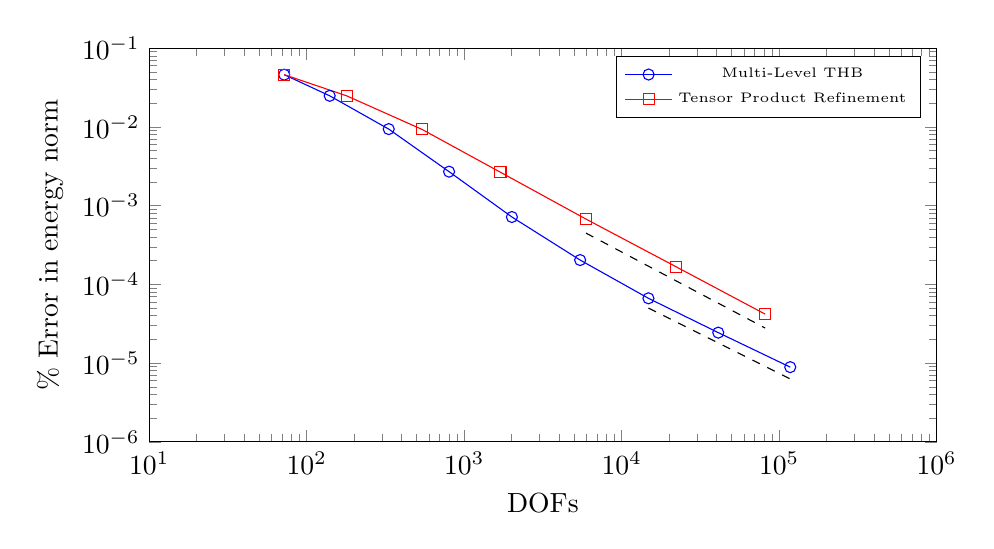
\begin{tikzpicture}

\begin{axis}[%
width=10cm,
height=5cm,
at={(0.758in,0.481in)},
scale only axis,
xmode=log,
xmin=1e1,
xmax=1e6,
xminorticks=true,
ymode=log,
ymin=1e-06,
ymax=0.1,
yminorticks=true,
axis background/.style={fill=white},
ylabel=\% Error in energy norm,
xlabel=DOFs,
legend style={font=\tiny}
]
\addplot [color=blue,solid,mark=o,mark options={solid}]
table[row sep=crcr]{%
	72	0.046063507578358\\
	140	0.024827123605165\\
	332	0.009376820174183\\
	802	0.002701826251341\\
	2010	0.000717396099949\\
	5450	0.000203703205243\\
	14798	6.6550742906e-05\\
	41072	2.4392674541e-05\\
	117666	8.891058362e-06\\
};
\addplot [color=black,dashed,forget plot]
table[row sep=crcr]{%
%	72	0.0102891419539127\\
%	140	0.00529155871915513\\
%	332	0.00223138018277626\\
%	802	0.000923713492121843\\
%	2010	0.000368566278946128\\
%	5450	0.000135929948748939\\
	14798	5.00620503231327e-05\\
	41072	1.80370622487758e-05\\
	117666	6.29594122925669e-06\\
};

\addplot [color=red,solid,mark=square,mark options={solid}]
table[row sep=crcr]{%
	72	0.046063507578358\\
	180	0.02474434964774\\
	540	0.009296481785437\\
	1700	0.002654912173056\\
	5940	0.000674787313856\\
	22100	0.000168011560559\\
	81528	4.1901685859e-05\\
};
\addplot [color=black,dashed,forget plot]
table[row sep=crcr]{%
%	72	0.0481580925080468\\
%	180	0.0182327789805753\\
%	540	0.00568989611811802\\
%	1700	0.00168719727846886\\
	5940	0.000447948504665927\\
	22100	0.000111272004773931\\
	81528	2.78905145726206e-05\\
};

\legend{Multi-Level THB, Tensor Product Refinement}

{
\logLogSlopeReverseTriangle{0.75}{0.05}{0.15}{1}{black};
\logLogSlopeTriangle{0.8}{0.05}{0.4}{1}{black};
}
\end{axis}
\end{tikzpicture}%
\end{frame}

\begin{frame}
	\frametitle{Example: Heat conduction on L-shape domain }%
	\begin{itemize}
		\item $ p=3 $
	\end{itemize}
	
	% This file was created by matlab2tikz.
%
%The latest updates can be retrieved from
%  http://www.mathworks.com/matlabcentral/fileexchange/22022-matlab2tikz-matlab2tikz
%where you can also make suggestions and rate matlab2tikz.
%

\pgfplotsset{compat=newest}

\usetikzlibrary{calc}

%%% START MACRO FOR ANNOTATION OF TRIANGLE WITH SLOPE %%%.
\newcommand{\logLogSlopeTriangle}[5]
{
	% #1. Relative offset in x direction.
	% #2. Width in x direction, so xA-xB.
	% #3. Relative offset in y direction.
	% #4. Slope d(y)/d(log10(x)).
	% #5. Plot options.
	
	\pgfplotsextra
	{
		\pgfkeysgetvalue{/pgfplots/xmin}{\xmin}
		\pgfkeysgetvalue{/pgfplots/xmax}{\xmax}
		\pgfkeysgetvalue{/pgfplots/ymin}{\ymin}
		\pgfkeysgetvalue{/pgfplots/ymax}{\ymax}
		
		% Calculate auxilliary quantities, in relative sense.
		\pgfmathsetmacro{\xArel}{#1}
		\pgfmathsetmacro{\yArel}{#3}
		\pgfmathsetmacro{\xBrel}{#1-#2}
		\pgfmathsetmacro{\yBrel}{\yArel}
		\pgfmathsetmacro{\xCrel}{\xArel}
		%\pgfmathsetmacro{\yCrel}{ln(\yC/exp(\ymin))/ln(exp(\ymax)/exp(\ymin))} % REPLACE THIS EXPRESSION WITH AN EXPRESSION INDEPENDENT OF \yC TO PREVENT THE 'DIMENSION TOO LARGE' ERROR.
		
		\pgfmathsetmacro{\lnxB}{\xmin*(1-(#1-#2))+\xmax*(#1-#2)} % in [xmin,xmax].
		\pgfmathsetmacro{\lnxA}{\xmin*(1-#1)+\xmax*#1} % in [xmin,xmax].
		\pgfmathsetmacro{\lnyA}{\ymin*(1-#3)+\ymax*#3} % in [ymin,ymax].
		\pgfmathsetmacro{\lnyC}{\lnyA-#4*(\lnxA-\lnxB)}
		\pgfmathsetmacro{\yCrel}{\lnyC-\ymin)/(\ymax-\ymin)}
		
		% Define coordinates for \draw. MIND THE 'rel axis cs' as opposed to the 'axis cs'.
		\coordinate (A) at (rel axis cs:\xArel,\yArel);
		\coordinate (B) at (rel axis cs:\xBrel,\yBrel);
		\coordinate (C) at (rel axis cs:\xCrel,\yCrel);
		
		% Draw slope triangle.
		\draw[#5]   (A)-- node[pos=0.5,anchor=south] {\scriptsize 1}
		(B)-- 
		(C)-- node[pos=0.5,anchor=west] {\scriptsize #4}
		cycle;
	}
}

\newcommand{\logLogSlopeReverseTriangle}[5]
{
	% #1. Relative offset in x direction.
	% #2. Width in x direction, so xA-xB.
	% #3. Relative offset in y direction.
	% #4. Slope d(y)/d(log10(x)).
	% #5. Plot options.
	
	\pgfplotsextra
	{
		\pgfkeysgetvalue{/pgfplots/xmin}{\xmin}
		\pgfkeysgetvalue{/pgfplots/xmax}{\xmax}
		\pgfkeysgetvalue{/pgfplots/ymin}{\ymin}
		\pgfkeysgetvalue{/pgfplots/ymax}{\ymax}
		
		% Calculate auxilliary quantities, in relative sense.
		\pgfmathsetmacro{\xArel}{#1}
		\pgfmathsetmacro{\yArel}{#3}
		\pgfmathsetmacro{\xBrel}{#1+#2}
		\pgfmathsetmacro{\yBrel}{\yArel}
		\pgfmathsetmacro{\xCrel}{\xArel}
		%\pgfmathsetmacro{\yCrel}{ln(\yC/exp(\ymin))/ln(exp(\ymax)/exp(\ymin))} % REPLACE THIS EXPRESSION WITH AN EXPRESSION INDEPENDENT OF \yC TO PREVENT THE 'DIMENSION TOO LARGE' ERROR.
		
		\pgfmathsetmacro{\lnxB}{\xmin*(1-(#1-#2))+\xmax*(#1-#2)} % in [xmin,xmax].
		\pgfmathsetmacro{\lnxA}{\xmin*(1-#1)+\xmax*#1} % in [xmin,xmax].
		\pgfmathsetmacro{\lnyA}{\ymin*(1-#3)+\ymax*#3} % in [ymin,ymax].
		\pgfmathsetmacro{\lnyC}{\lnyA+#4*(\lnxA-\lnxB)}
		\pgfmathsetmacro{\yCrel}{\lnyC-\ymin)/(\ymax-\ymin)}
		
		% Define coordinates for \draw. MIND THE 'rel axis cs' as opposed to the 'axis cs'.
		\coordinate (A) at (rel axis cs:\xArel,\yArel);
		\coordinate (B) at (rel axis cs:\xBrel,\yBrel);
		\coordinate (C) at (rel axis cs:\xCrel,\yCrel);
		
		% Draw slope triangle.
		\draw[#5]   (A)-- node[pos=0.5,anchor=north] {\scriptsize 1}
		(B)-- 
		(C)-- node[pos=0.5,anchor=east] {\scriptsize #4}
		cycle;
	}
}
%%% END MACRO FOR ANNOTATION OF TRIANGLE WITH SLOPE %%%.


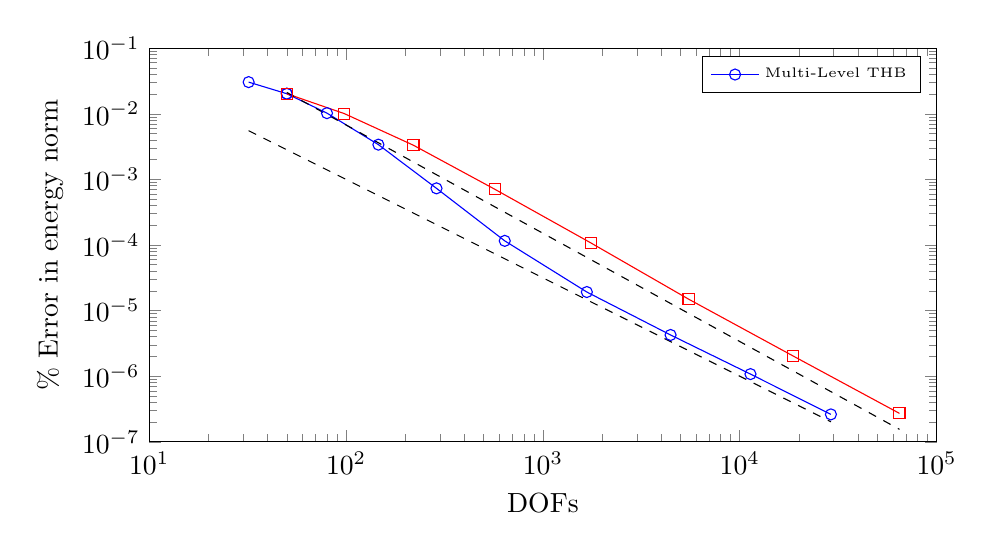
\begin{tikzpicture}

\begin{axis}[%
width=10cm,
height=5cm,
at={(0.758in,0.481in)},
scale only axis,
xmode=log,
xmin=1e1,
xmax=1e5,
xminorticks=true,
ymode=log,
ymin=1e-07,
ymax=0.1,
yminorticks=true,
axis background/.style={fill=white},
ylabel=\% Error in energy norm,
xlabel=DOFs,
legend style={font=\tiny}
]
%\addplot [color=blue,solid,mark=o,mark options={solid}]
\addplot [color=blue,solid,mark=o,mark options={solid}]
table[row sep=crcr]{%
	50	0.020215407314022\\
%	48	0.0500073829665119\\
%	76	0.0278449560820008\\
%	142	0.0126970619240542\\
%	242	0.00660733441696399\\
%	312	0.00435668459205658\\
%	552	0.00255759420607355\\
%	796	0.00151589672287713\\
%	1236	0.000944445092205633\\
%	2074	0.000566215208140263\\
%	3146	0.000339514546405781\\
%	4640	0.000241941547691511\\
%	8126	0.000134548935705695\\
%	11536	8.70810027272917e-05\\
%	16760	6.25408392329503e-05\\
};

\addplot [color=blue,solid,mark=o,mark options={solid},forget plot]
table[row sep=crcr]{%
	32	0.030377298795457\\
	50	0.020215407314022\\
	80	0.01022813148539\\
	146	0.003385914241628\\
	288	0.000730736277324\\
	640	0.000115704036217\\
	1672	1.9205964552e-05\\
	4452	4.256999848e-06\\
	11334	1.078521451e-06\\
	29044	2.62217932e-07\\
};
\addplot [color=black,dashed,forget plot]
table[row sep=crcr]{%
	32	0.0055242717280199\\
	50	0.00282842712474619\\
	80	0.00139754248593737\\
	146	0.000566853348357786\\
	288	0.00020460265659333\\
	640	6.17632355501637e-05\\
	1672	1.46266742836279e-05\\
	4452	3.36641200207873e-06\\
	11334	8.28753141260167e-07\\
	29044	2.02029764629279e-07\\
};

\addplot [color=red,solid,mark=square,mark options={solid},forget plot]
table[row sep=crcr]{%
	50	0.020215407314022\\
	98	0.010061106355559\\
	220	0.00331363837803\\
	570	0.000707169451588\\
	1750	0.000107903131278\\
	5494	1.4973311526e-05\\
	18602	2.047466221e-06\\
	64750	2.71695565e-07\\
};
\addplot [color=black,dashed,forget plot]
table[row sep=crcr]{%
	50	0.0211770345808887\\
	98	0.00697658079409742\\
	220	0.00183724988806352\\
	570	0.000381919770850579\\
	1750	6.00002241201106e-05\\
	5494	9.08551128307312e-06\\
	18602	1.21448525627835e-06\\
	64750	1.5510293924838e-07\\
};


\legend{Multi-Level THB, Tensor Product Refinement}

{
\logLogSlopeReverseTriangle{0.77}{0.05}{0.08}{1.5}{black};
\logLogSlopeTriangle{0.93}{0.05}{0.115}{1.65}{black};
}
\end{axis}
\end{tikzpicture}%
\end{frame}

\begin{frame}
	\frametitle{Example: (Linear) elastic plate with circular hole }%
	$ \sigma_{XX} $, control mesh and B\`ezier control mesh obtained by the multi-level B\`ezier extraction operator ($ p=2 $)\\
	\centering
	\begin{minipage}{0.49\textwidth}
		\centering
		\includegraphics[scale=0.24]{pics/plateWithAHole/plate_beziernet_1.png}
	\end{minipage}
	\begin{minipage}{0.49\textwidth}
		\centering
		\includegraphics[scale=0.24]{pics/plateWithAHole/plate_controlnet_1.png}
	\end{minipage}
\end{frame}

\begin{frame}
	\frametitle{Example: (Linear) elastic plate with circular hole }%
	Control mesh and B\`ezier control mesh obtained by the multi-level B\`ezier extraction operator ($ p=2 $)\\
	\centering
	\begin{minipage}{0.49\textwidth}
		\centering
		\includegraphics[scale=0.24]{pics/plateWithAHole/plate_beziernet_2.png}
	\end{minipage}
	\begin{minipage}{0.49\textwidth}
		\centering
		\includegraphics[scale=0.24]{pics/plateWithAHole/plate_controlnet_2.png}
	\end{minipage}
\end{frame}

\begin{frame}
	\frametitle{Example: (Linear) elastic plate with circular hole }%
	Control mesh and B\`ezier control mesh obtained by the multi-level B\`ezier extraction operator ($ p=2 $)\\
	\centering
	\begin{minipage}{0.49\textwidth}
		\centering
		\includegraphics[scale=0.24]{pics/plateWithAHole/plate_beziernet_3.png}
	\end{minipage}
	\begin{minipage}{0.49\textwidth}
		\centering
		\includegraphics[scale=0.24]{pics/plateWithAHole/plate_controlnet_3.png}
	\end{minipage}
\end{frame}

\begin{frame}
	\frametitle{Example: (Linear) elastic plate with circular hole }%
	\begin{itemize}
		\item $ p=2 $
	\end{itemize}
	% This file was created by matlab2tikz.
%
%The latest updates can be retrieved from
%  http://www.mathworks.com/matlabcentral/fileexchange/22022-matlab2tikz-matlab2tikz
%where you can also make suggestions and rate matlab2tikz.
%

\pgfplotsset{compat=newest}

\usetikzlibrary{calc}

%%% START MACRO FOR ANNOTATION OF TRIANGLE WITH SLOPE %%%.
\newcommand{\logLogSlopeTriangle}[5]
{
	% #1. Relative offset in x direction.
	% #2. Width in x direction, so xA-xB.
	% #3. Relative offset in y direction.
	% #4. Slope d(y)/d(log10(x)).
	% #5. Plot options.
	
	\pgfplotsextra
	{
		\pgfkeysgetvalue{/pgfplots/xmin}{\xmin}
		\pgfkeysgetvalue{/pgfplots/xmax}{\xmax}
		\pgfkeysgetvalue{/pgfplots/ymin}{\ymin}
		\pgfkeysgetvalue{/pgfplots/ymax}{\ymax}
		
		% Calculate auxilliary quantities, in relative sense.
		\pgfmathsetmacro{\xArel}{#1}
		\pgfmathsetmacro{\yArel}{#3}
		\pgfmathsetmacro{\xBrel}{#1-#2}
		\pgfmathsetmacro{\yBrel}{\yArel}
		\pgfmathsetmacro{\xCrel}{\xArel}
		%\pgfmathsetmacro{\yCrel}{ln(\yC/exp(\ymin))/ln(exp(\ymax)/exp(\ymin))} % REPLACE THIS EXPRESSION WITH AN EXPRESSION INDEPENDENT OF \yC TO PREVENT THE 'DIMENSION TOO LARGE' ERROR.
		
		\pgfmathsetmacro{\lnxB}{\xmin*(1-(#1-#2))+\xmax*(#1-#2)} % in [xmin,xmax].
		\pgfmathsetmacro{\lnxA}{\xmin*(1-#1)+\xmax*#1} % in [xmin,xmax].
		\pgfmathsetmacro{\lnyA}{\ymin*(1-#3)+\ymax*#3} % in [ymin,ymax].
		\pgfmathsetmacro{\lnyC}{\lnyA-#4*(\lnxA-\lnxB)}
		\pgfmathsetmacro{\yCrel}{\lnyC-\ymin)/(\ymax-\ymin)}
		
		% Define coordinates for \draw. MIND THE 'rel axis cs' as opposed to the 'axis cs'.
		\coordinate (A) at (rel axis cs:\xArel,\yArel);
		\coordinate (B) at (rel axis cs:\xBrel,\yBrel);
		\coordinate (C) at (rel axis cs:\xCrel,\yCrel);
		
		% Draw slope triangle.
		\draw[#5]   (A)-- node[pos=0.5,anchor=south] {\scriptsize 1}
		(B)-- 
		(C)-- node[pos=0.5,anchor=west] {\scriptsize #4}
		cycle;
	}
}

\newcommand{\logLogSlopeReverseTriangle}[5]
{
	% #1. Relative offset in x direction.
	% #2. Width in x direction, so xA-xB.
	% #3. Relative offset in y direction.
	% #4. Slope d(y)/d(log10(x)).
	% #5. Plot options.
	
	\pgfplotsextra
	{
		\pgfkeysgetvalue{/pgfplots/xmin}{\xmin}
		\pgfkeysgetvalue{/pgfplots/xmax}{\xmax}
		\pgfkeysgetvalue{/pgfplots/ymin}{\ymin}
		\pgfkeysgetvalue{/pgfplots/ymax}{\ymax}
		
		% Calculate auxilliary quantities, in relative sense.
		\pgfmathsetmacro{\xArel}{#1}
		\pgfmathsetmacro{\yArel}{#3}
		\pgfmathsetmacro{\xBrel}{#1+#2}
		\pgfmathsetmacro{\yBrel}{\yArel}
		\pgfmathsetmacro{\xCrel}{\xArel}
		%\pgfmathsetmacro{\yCrel}{ln(\yC/exp(\ymin))/ln(exp(\ymax)/exp(\ymin))} % REPLACE THIS EXPRESSION WITH AN EXPRESSION INDEPENDENT OF \yC TO PREVENT THE 'DIMENSION TOO LARGE' ERROR.
		
		\pgfmathsetmacro{\lnxB}{\xmin*(1-(#1-#2))+\xmax*(#1-#2)} % in [xmin,xmax].
		\pgfmathsetmacro{\lnxA}{\xmin*(1-#1)+\xmax*#1} % in [xmin,xmax].
		\pgfmathsetmacro{\lnyA}{\ymin*(1-#3)+\ymax*#3} % in [ymin,ymax].
		\pgfmathsetmacro{\lnyC}{\lnyA+#4*(\lnxA-\lnxB)}
		\pgfmathsetmacro{\yCrel}{\lnyC-\ymin)/(\ymax-\ymin)}
		
		% Define coordinates for \draw. MIND THE 'rel axis cs' as opposed to the 'axis cs'.
		\coordinate (A) at (rel axis cs:\xArel,\yArel);
		\coordinate (B) at (rel axis cs:\xBrel,\yBrel);
		\coordinate (C) at (rel axis cs:\xCrel,\yCrel);
		
		% Draw slope triangle.
		\draw[#5]   (A)-- node[pos=0.5,anchor=north] {\scriptsize 1}
		(B)-- 
		(C)-- node[pos=0.5,anchor=east] {\scriptsize #4}
		cycle;
	}
}
%%% END MACRO FOR ANNOTATION OF TRIANGLE WITH SLOPE %%%.


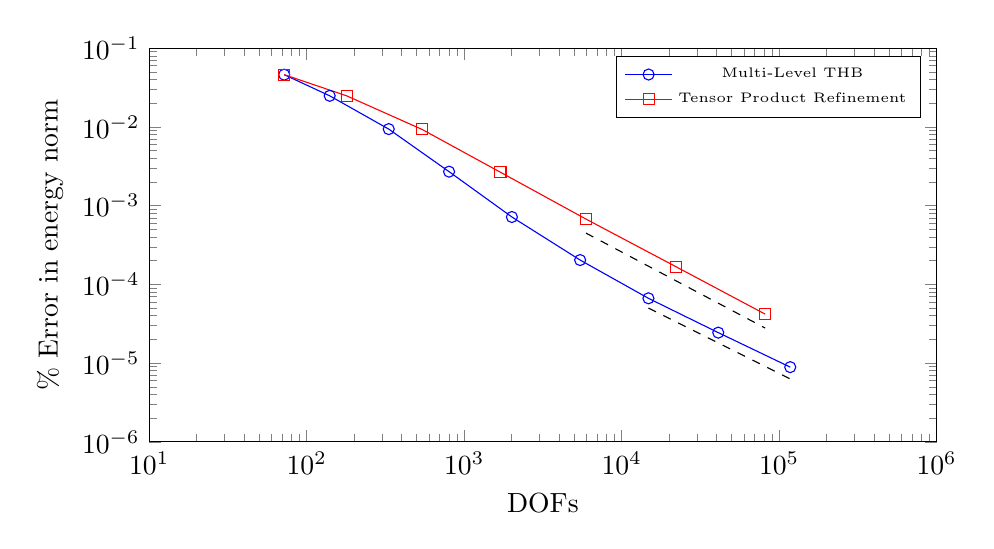
\begin{tikzpicture}

\begin{axis}[%
width=10cm,
height=5cm,
at={(0.758in,0.481in)},
scale only axis,
xmode=log,
xmin=1e1,
xmax=1e6,
xminorticks=true,
ymode=log,
ymin=1e-06,
ymax=0.1,
yminorticks=true,
axis background/.style={fill=white},
ylabel=\% Error in energy norm,
xlabel=DOFs,
legend style={font=\tiny}
]
\addplot [color=blue,solid,mark=o,mark options={solid}]
table[row sep=crcr]{%
	72	0.046063507578358\\
	140	0.024827123605165\\
	332	0.009376820174183\\
	802	0.002701826251341\\
	2010	0.000717396099949\\
	5450	0.000203703205243\\
	14798	6.6550742906e-05\\
	41072	2.4392674541e-05\\
	117666	8.891058362e-06\\
};
\addplot [color=black,dashed,forget plot]
table[row sep=crcr]{%
%	72	0.0102891419539127\\
%	140	0.00529155871915513\\
%	332	0.00223138018277626\\
%	802	0.000923713492121843\\
%	2010	0.000368566278946128\\
%	5450	0.000135929948748939\\
	14798	5.00620503231327e-05\\
	41072	1.80370622487758e-05\\
	117666	6.29594122925669e-06\\
};

\addplot [color=red,solid,mark=square,mark options={solid}]
table[row sep=crcr]{%
	72	0.046063507578358\\
	180	0.02474434964774\\
	540	0.009296481785437\\
	1700	0.002654912173056\\
	5940	0.000674787313856\\
	22100	0.000168011560559\\
	81528	4.1901685859e-05\\
};
\addplot [color=black,dashed,forget plot]
table[row sep=crcr]{%
%	72	0.0481580925080468\\
%	180	0.0182327789805753\\
%	540	0.00568989611811802\\
%	1700	0.00168719727846886\\
	5940	0.000447948504665927\\
	22100	0.000111272004773931\\
	81528	2.78905145726206e-05\\
};

\legend{Multi-Level THB, Tensor Product Refinement}

{
\logLogSlopeReverseTriangle{0.75}{0.05}{0.15}{1}{black};
\logLogSlopeTriangle{0.8}{0.05}{0.4}{1}{black};
}
\end{axis}
\end{tikzpicture}%
\end{frame}

\begin{frame}
	\frametitle{Example: (Linear) elastic plate with circular hole }%
	\begin{itemize}
		\item $ p=3 $
	\end{itemize}
	% This file was created by matlab2tikz.
%
%The latest updates can be retrieved from
%  http://www.mathworks.com/matlabcentral/fileexchange/22022-matlab2tikz-matlab2tikz
%where you can also make suggestions and rate matlab2tikz.
%

\pgfplotsset{compat=newest}

\usetikzlibrary{calc}

%%% START MACRO FOR ANNOTATION OF TRIANGLE WITH SLOPE %%%.
\newcommand{\logLogSlopeTriangle}[5]
{
	% #1. Relative offset in x direction.
	% #2. Width in x direction, so xA-xB.
	% #3. Relative offset in y direction.
	% #4. Slope d(y)/d(log10(x)).
	% #5. Plot options.
	
	\pgfplotsextra
	{
		\pgfkeysgetvalue{/pgfplots/xmin}{\xmin}
		\pgfkeysgetvalue{/pgfplots/xmax}{\xmax}
		\pgfkeysgetvalue{/pgfplots/ymin}{\ymin}
		\pgfkeysgetvalue{/pgfplots/ymax}{\ymax}
		
		% Calculate auxilliary quantities, in relative sense.
		\pgfmathsetmacro{\xArel}{#1}
		\pgfmathsetmacro{\yArel}{#3}
		\pgfmathsetmacro{\xBrel}{#1-#2}
		\pgfmathsetmacro{\yBrel}{\yArel}
		\pgfmathsetmacro{\xCrel}{\xArel}
		%\pgfmathsetmacro{\yCrel}{ln(\yC/exp(\ymin))/ln(exp(\ymax)/exp(\ymin))} % REPLACE THIS EXPRESSION WITH AN EXPRESSION INDEPENDENT OF \yC TO PREVENT THE 'DIMENSION TOO LARGE' ERROR.
		
		\pgfmathsetmacro{\lnxB}{\xmin*(1-(#1-#2))+\xmax*(#1-#2)} % in [xmin,xmax].
		\pgfmathsetmacro{\lnxA}{\xmin*(1-#1)+\xmax*#1} % in [xmin,xmax].
		\pgfmathsetmacro{\lnyA}{\ymin*(1-#3)+\ymax*#3} % in [ymin,ymax].
		\pgfmathsetmacro{\lnyC}{\lnyA-#4*(\lnxA-\lnxB)}
		\pgfmathsetmacro{\yCrel}{\lnyC-\ymin)/(\ymax-\ymin)}
		
		% Define coordinates for \draw. MIND THE 'rel axis cs' as opposed to the 'axis cs'.
		\coordinate (A) at (rel axis cs:\xArel,\yArel);
		\coordinate (B) at (rel axis cs:\xBrel,\yBrel);
		\coordinate (C) at (rel axis cs:\xCrel,\yCrel);
		
		% Draw slope triangle.
		\draw[#5]   (A)-- node[pos=0.5,anchor=south] {\scriptsize 1}
		(B)-- 
		(C)-- node[pos=0.5,anchor=west] {\scriptsize #4}
		cycle;
	}
}

\newcommand{\logLogSlopeReverseTriangle}[5]
{
	% #1. Relative offset in x direction.
	% #2. Width in x direction, so xA-xB.
	% #3. Relative offset in y direction.
	% #4. Slope d(y)/d(log10(x)).
	% #5. Plot options.
	
	\pgfplotsextra
	{
		\pgfkeysgetvalue{/pgfplots/xmin}{\xmin}
		\pgfkeysgetvalue{/pgfplots/xmax}{\xmax}
		\pgfkeysgetvalue{/pgfplots/ymin}{\ymin}
		\pgfkeysgetvalue{/pgfplots/ymax}{\ymax}
		
		% Calculate auxilliary quantities, in relative sense.
		\pgfmathsetmacro{\xArel}{#1}
		\pgfmathsetmacro{\yArel}{#3}
		\pgfmathsetmacro{\xBrel}{#1+#2}
		\pgfmathsetmacro{\yBrel}{\yArel}
		\pgfmathsetmacro{\xCrel}{\xArel}
		%\pgfmathsetmacro{\yCrel}{ln(\yC/exp(\ymin))/ln(exp(\ymax)/exp(\ymin))} % REPLACE THIS EXPRESSION WITH AN EXPRESSION INDEPENDENT OF \yC TO PREVENT THE 'DIMENSION TOO LARGE' ERROR.
		
		\pgfmathsetmacro{\lnxB}{\xmin*(1-(#1-#2))+\xmax*(#1-#2)} % in [xmin,xmax].
		\pgfmathsetmacro{\lnxA}{\xmin*(1-#1)+\xmax*#1} % in [xmin,xmax].
		\pgfmathsetmacro{\lnyA}{\ymin*(1-#3)+\ymax*#3} % in [ymin,ymax].
		\pgfmathsetmacro{\lnyC}{\lnyA+#4*(\lnxA-\lnxB)}
		\pgfmathsetmacro{\yCrel}{\lnyC-\ymin)/(\ymax-\ymin)}
		
		% Define coordinates for \draw. MIND THE 'rel axis cs' as opposed to the 'axis cs'.
		\coordinate (A) at (rel axis cs:\xArel,\yArel);
		\coordinate (B) at (rel axis cs:\xBrel,\yBrel);
		\coordinate (C) at (rel axis cs:\xCrel,\yCrel);
		
		% Draw slope triangle.
		\draw[#5]   (A)-- node[pos=0.5,anchor=north] {\scriptsize 1}
		(B)-- 
		(C)-- node[pos=0.5,anchor=east] {\scriptsize #4}
		cycle;
	}
}
%%% END MACRO FOR ANNOTATION OF TRIANGLE WITH SLOPE %%%.


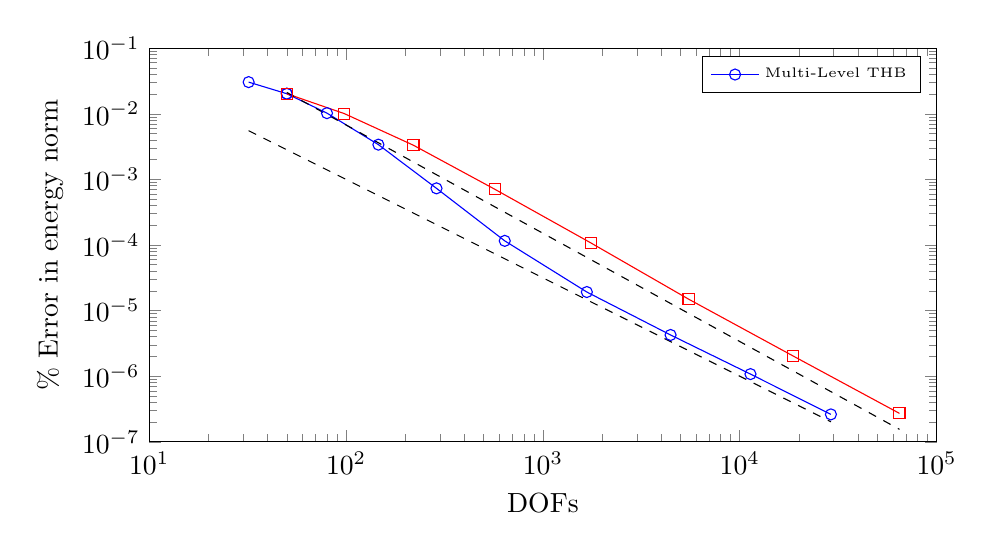
\begin{tikzpicture}

\begin{axis}[%
width=10cm,
height=5cm,
at={(0.758in,0.481in)},
scale only axis,
xmode=log,
xmin=1e1,
xmax=1e5,
xminorticks=true,
ymode=log,
ymin=1e-07,
ymax=0.1,
yminorticks=true,
axis background/.style={fill=white},
ylabel=\% Error in energy norm,
xlabel=DOFs,
legend style={font=\tiny}
]
%\addplot [color=blue,solid,mark=o,mark options={solid}]
\addplot [color=blue,solid,mark=o,mark options={solid}]
table[row sep=crcr]{%
	50	0.020215407314022\\
%	48	0.0500073829665119\\
%	76	0.0278449560820008\\
%	142	0.0126970619240542\\
%	242	0.00660733441696399\\
%	312	0.00435668459205658\\
%	552	0.00255759420607355\\
%	796	0.00151589672287713\\
%	1236	0.000944445092205633\\
%	2074	0.000566215208140263\\
%	3146	0.000339514546405781\\
%	4640	0.000241941547691511\\
%	8126	0.000134548935705695\\
%	11536	8.70810027272917e-05\\
%	16760	6.25408392329503e-05\\
};

\addplot [color=blue,solid,mark=o,mark options={solid},forget plot]
table[row sep=crcr]{%
	32	0.030377298795457\\
	50	0.020215407314022\\
	80	0.01022813148539\\
	146	0.003385914241628\\
	288	0.000730736277324\\
	640	0.000115704036217\\
	1672	1.9205964552e-05\\
	4452	4.256999848e-06\\
	11334	1.078521451e-06\\
	29044	2.62217932e-07\\
};
\addplot [color=black,dashed,forget plot]
table[row sep=crcr]{%
	32	0.0055242717280199\\
	50	0.00282842712474619\\
	80	0.00139754248593737\\
	146	0.000566853348357786\\
	288	0.00020460265659333\\
	640	6.17632355501637e-05\\
	1672	1.46266742836279e-05\\
	4452	3.36641200207873e-06\\
	11334	8.28753141260167e-07\\
	29044	2.02029764629279e-07\\
};

\addplot [color=red,solid,mark=square,mark options={solid},forget plot]
table[row sep=crcr]{%
	50	0.020215407314022\\
	98	0.010061106355559\\
	220	0.00331363837803\\
	570	0.000707169451588\\
	1750	0.000107903131278\\
	5494	1.4973311526e-05\\
	18602	2.047466221e-06\\
	64750	2.71695565e-07\\
};
\addplot [color=black,dashed,forget plot]
table[row sep=crcr]{%
	50	0.0211770345808887\\
	98	0.00697658079409742\\
	220	0.00183724988806352\\
	570	0.000381919770850579\\
	1750	6.00002241201106e-05\\
	5494	9.08551128307312e-06\\
	18602	1.21448525627835e-06\\
	64750	1.5510293924838e-07\\
};


\legend{Multi-Level THB, Tensor Product Refinement}

{
\logLogSlopeReverseTriangle{0.77}{0.05}{0.08}{1.5}{black};
\logLogSlopeTriangle{0.93}{0.05}{0.115}{1.65}{black};
}
\end{axis}
\end{tikzpicture}%
\end{frame}



%------------------------------------------------

%\begin{frame}
%\Huge{\centerline{The End}}
%\end{frame}

%----------------------------------------------------------------------------------------

\end{document} 